\documentclass{article}

\usepackage{Mathematics}
\pdftitle{Mathematics 3A}

% === TITLE ===
\title{\textbf{Mathematics 3A \\ HSLU, Semester 3}}
\author{Matteo Frongillo}
\date{}

% === TEXT ===
\begin{document}

\maketitle
\tableofcontents
\pagebreak

\part{Just stuff I have to explain, wait few days}
Let $\pi$ denote the plane:
\[s_y\in \pi, s_y\in\pi, s_z\in\pi\]
\[\pi: ax+by+cz+d=0\qquad \]

For $S_x\in\pi \Longrightarrow 1a+0b+0c+d = 0$, hence\\
$a+d=0$

For $S_y\in\pi \Longrightarrow 0a+2b+0c+d=0$, hence\\
$2b+d=0$

for $S_z\in\pi \Longrightarrow 0a+0b+3c+d=0$, hence\\
$3c+d=0$

\[
\begin{cases}
    a+d=0\\
    2b+d=0\\
    3c+d=0
\end{cases}
\Longrightarrow
\begin{cases}
    a=-d\\
    2b=-d\\
    3c=-d
\end{cases}
\]

Case 1:
\[d=0 \Longrightarrow a=0, b=0, c=0 \Longrightarrow \pi: 0=0 \Longrightarrow \text{NOT a plane!}\]

Case 2:
\[d\neq0 \Longrightarrow \pi:\frac{ax+by+cz+d}{d} = 0 \Longrightarrow \frac{a}{d}x + \frac{b}{d}y + \frac{c}{d}z + 1 = 0\]

Hence:
\[
\begin{cases}
    a=-d\\
    2b=-d\\
    3c=-d
\end{cases}
\Longrightarrow
\begin{cases}
    \frac{a}{d} = -1\\
    \frac{b}{d} = -\frac{1}{2}\\
    \frac{c}{d} = -\frac{1}{3}
\end{cases}
\]

Which leads to:
\[\pi: -x-\frac{1}{2}y-\frac{1}{3}z + 1 = 0\]

\rem{the equation of a plane is defined up to a multiplication by a real number different from 0}

e.g.: the same planed is shared between those 3 equations\\
ex 1)
\[z=0 \Longleftrightarrow 5z=0 \Longleftrightarrow -10z=0\]

ex 2)
\[-x-\frac{1}{2}y-\frac{1}{3}z + 1 = 0 \Longleftrightarrow 6x+3y+2z+6=0\]


\newpage
\section{Functions in two variables $x$ and $y$}
Let us take $\pi:x^2-y^2=0$ as example.

The plot would look like this:

\begin{center}
    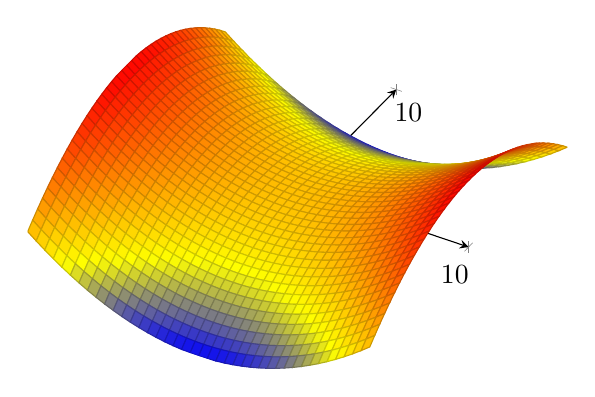
\begin{tikzpicture}
      \begin{axis}[view={30}{60}, axis lines=middle, domain=-10:10, y domain=-10:10, samples=41]
        \addplot3[surf] {x^2 - y^2};
      \end{axis}
    \end{tikzpicture}
\end{center}

\subsection{Spheres}









\end{document}